% This is samplepaper.tex, a sample chapter demonstrating the
% LLNCS macro package for Springer Computer Science proceedings;
% Version 2.20 of 2017/10/04
%
\documentclass[runningheads]{llncs}
%
\usepackage{graphicx}
\usepackage[ruled,vlined]{algorithm2e}
\usepackage{hyperref}\usepackage{amsmath}
\usepackage{todonotes}

% Used for displaying a sample figure. If possible, figure files should
% be included in EPS format.
%
% If you use the hyperref package, please uncomment the following line
% to display URLs in blue roman font according to Springer's eBook style:
\renewcommand\UrlFont{\color{blue}\rmfamily}

\begin{document}
%
\title{Machine Learning for Computer Vision}
\subtitle{Image classification}
%
%\titlerunning{Abbreviated paper title}
% If the paper title is too long for the running head, you can set
% an abbreviated paper title here
%
\author{Roger Casals Vilardell\inst{1}, Pau Domingo Gregorio\inst{1}, Joan Fontanals Martinez\inst{1}}
%
\authorrunning{R.Casals, P.Domingo, J. Fontanals}
% First names are abbreviated in the running head.
% If there are more than two authors, 'et al.' is used.
%
\institute{Computer Vision Center, Universitat Autonoma de Barcelona
\email{rogercasalsvilardell@gmail.com, pavdom72@gmail.com, jfontanalsmartinez@gmail.com}}
%
\maketitle              % typeset the header of the contribution
%
\begin{abstract}
Image classification is a classical problem in which a system is designed to classify images into a set of classes. This problem can be addressed using multiple techniques, from using classical computer vision descriptor and techniques to the latest advanced deep learning based methods.
In this document an image classification system is built by using different approaches and tools. It starts addressing the problem with a Bag of Visual Words approach supported by some machine learning techniques, to end introducing the use of Deep Learning by using Convolutional Neural Networks to provide a set of learned features or to apply Transfer Learning from a different classification problem. Finally, a new architecture is proposed that tries to obtain the best possible accuracy while maintaining a compact structure to minimize the number of parameters to learn. The aim of this project is also to analyze the benefits provided for each method. \todo{1. remove this cite now just useful to avoid compile warning}\cite{opencv_library}

\keywords{Image classification \and Deep Learning  \and Computer Vision}
\end{abstract}

\section{Problem description} \label{problem}
The goal of this project is to classify a set of landscape images into 8 different classes.
These classes are: Coast, Forest, Highway, Inside city, Mountain, Open country, Street or Tall building. 
\begin{figure}
  \centering
  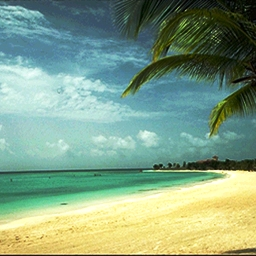
\includegraphics[width=.2\textwidth]{coast.jpg}\hfill
  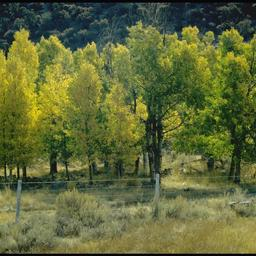
\includegraphics[width=.2\textwidth]{forest.jpg}\hfill
  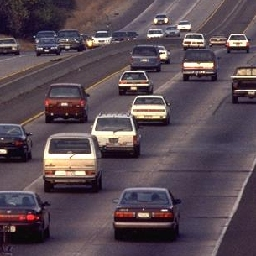
\includegraphics[width=.2\textwidth]{highway.jpg}\hfill
  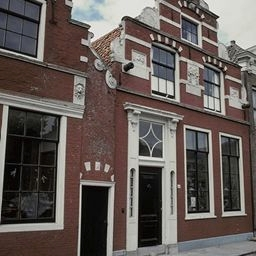
\includegraphics[width=.2\textwidth]{city.jpg}
  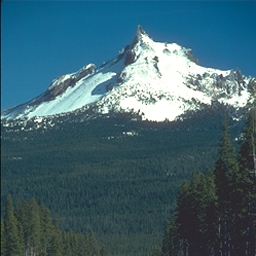
\includegraphics[width=.2\textwidth]{mountain.jpg}\hfill
  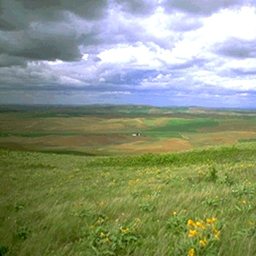
\includegraphics[width=.2\textwidth]{opencountry.jpg}\hfill
  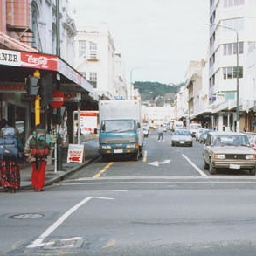
\includegraphics[width=.2\textwidth]{street.jpg}\hfill
  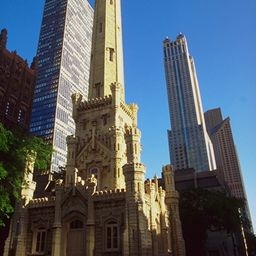
\includegraphics[width=.2\textwidth]{tallbuilding.jpg}
  \caption{Example of images per class}
\end{figure}
\todo{2. Proper order and comment image}

In order to develop the system implementing the task 1881 training samples are provided distributed among these classes. 
The performance of the system obtained is computed on 807 images belonging to these classes but which are different to the ones used during the training process of the system.

The project is structured to detail the steps followed to get the final system. The project covers:
\todo{3. Refine this list, (maybe style)}
\begin{itemize}
	\item Bag of Visual Words framework
	\item Use of K-Nearest Neighbours algorithm
	\item Use of Support Vector Machines
	\item Extract from a Multi Layer Neural Network
	\item Transfer learning from a system developed to solve a different domain problem
	\item Design a full CNN architecture
\end{itemize}

\section{Methods and Procedures}
\subsection{Bag of Visual Words (BOvW) framework} \label{BOvW}

In traditional computer vision techniques, local features such as SIFT or SURF \todo{4. Cite something about SIFT or SURF} are used to represent images for image categorization. Matching key-point's features based on similarity was the global framework to tackle these challenges.

These approaches face major issues, mostly because of the computational cost and the dimensionality of the features extracted.

Bag-of-Visual-words tries to obtain a global fixed-length vector representation of every image. It is a method inspired by the Bag-of-Words model used in Natural Language Processing, which is a popular framework for text classification.
\todo{5. Add citation to paper explaining Bag of Words in NLP}

The main idea is that a document can be described by a histogram vector representing the number of appearances of a word in a document. So, for instance, documents with many appearances of words such as vision, eye, camera, etc ... can later be potentially categorized into Computer Vision text. The main problem it faces is the design of the vocabulary that contains all the words taken into account.

Similarly, Bag-Of-Visual-Words tries to build a vocabulary of features that is counted in an histogram for each image and which becomes its fixed-length vector representation.

First, it is necessary to find a vocabulary of image features, in order to have a low-dimensional global representation of the image. This vocabulary is computed by training a K-Means algorithm fed with all the local features (SIFT in this case) computed for all the key-points of tall the images.

Once the K-Means algorithm is trained, every key-point descriptor is projected onto its visual word. Then, every image can compute an histogram of visual words that represents its global descriptor.
\todo{6. Image comparing pyramid with one global representation}
Another variant of this method is to split the images into some parts, and apply this analysis for each part individually. Afterwards, all the part's histograms are concatenated to have the global descriptor.

\todo{7. Add math equations and things about K-Means, local features turning into one single global vector features per image}

Given the small amount of data available for training, it may be necessary to consider the option to do some dimensionality reduction of the feature space, in order to help the system regularize better.

During this project, in the BOvW framework, the features to build the vocabulary are the ones computed using the DenseSIFT, or the version of it which is called in this project PyramidSIFT in which features of different parts of the image are computed independently to be combined into a global image representation. \todo{8. Cite something about DenseSIFT}. Two different dimensionality reduction techniques have been tested, Principal Component Analysis (PCA) and Linear Discriminant Analysis (LDA).
\todo{9. Cite some work related to these PCA dnd LDA}

\subsection{K-Nearest Neighbors}

The first method used for the classification tests is to use the K-Nearest Neighbors algorithms.
In K-Nearest Neighbors classification is computed from a majority vote of the nearest neighbors of each point.
An image will be assigned the class of the majority of its k-nearest neighbors in the training set of images.

The precision of this method depends basically on two factors. The number of neighbors considered and the distance metric.

The results can be found in \ref{KNNResults}

\todo{10. Put real results here}
\begin{table}[ht!]
\caption{Results of KNN .}
\begin{center}
\begin{tabular}{ | c | c | c | c | }
\hline
 & \textbf{Map at 1} & \textbf{Map a 3} & \textbf{F} \\ 
 \hline
 \textbf{Color descriptor} & 0.6 & 0.7 & 0.4 \\  
 \hline
 \textbf{LBP descriptor} & 0.7 & 0.75 & 0.5 \\ 
 \hline
 \textbf{HOG descriptor} & 0.8 & 0.85 & 0.6 \\  
 \hline
 \textbf{Combined descriptors} & 0.95 & 0.98 & 0.8 \\  
 \hline
\end{tabular}
\label{KNNResults}
\end{center}
\end{table}

\subsection{Support Vector Machines (SVM)}

Support Vector Machines is a supervised machine learning algorithm that tries to find two hyper-planes that separate two data-sets with the largest margin possible. 

\begin{figure}
  \centering
  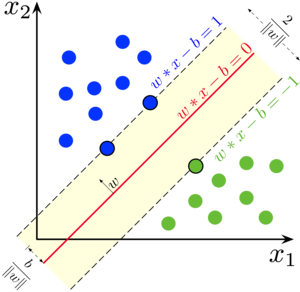
\includegraphics[width=0.5\textwidth]{SVM.png}\hfill
  \caption{SVM works by finding an hyper-planes that separates two different class data-sets with the maximal margin possible}
\end{figure}

In order to accomplish this task, it is needed to solve the Quadratic Constrained Optimization problem defined by: 
\todo{12. Put here equations about the maximization problem}

Since this is a Quadratic Problem, this problem can be rewritten into its prime Lagrangian form as:
\todo{13. Put here Lagrangian equation}

Those LAMBDA parameters \todo{14. change lambda by the symbol} different than 0, will define the set of training samples (the support vectors) that define the separating hyper-planes.

The prime problem described in \todo{15. reference prime Lagrangian equation} can be written in the dual form:
\todo{16. Put here dual form}

To solve the dual form, train samples are projected into another space defined by the projection function FUNC(X) \todo{17. change this FUNC(X)}. But for the solution of the optimization problem, it is not needed to find the exact transformation function, it is enough to know the value of the scalar product in that new space. This is known as the Kernel trick. \todo{18. Cite some paper about the Kernel trick, or SVMs in general}

SVM is tested as a solution to solve the proposed problem. The main challenge to make it work is to find the best Kernel function and to tweak the regularization parameter C, that allows for some flexibility to have some training samples between the dividing hyper-planes.

The results of training the SVM with features computed using the Bag-Of-Visual-Words framework can be found in \ref{SVMResults}

\todo{19. Put real results here}
\begin{table}[ht!]
\caption{Results of SVM with BOvW features .}
\begin{center}
\begin{tabular}{ | c | c | c | c | }
\hline
 & \textbf{Map at 1} & \textbf{Map a 3} & \textbf{F} \\ 
 \hline
 \textbf{Color descriptor} & 0.6 & 0.7 & 0.4 \\  
 \hline
 \textbf{LBP descriptor} & 0.7 & 0.75 & 0.5 \\ 
 \hline
 \textbf{HOG descriptor} & 0.8 & 0.85 & 0.6 \\  
 \hline
 \textbf{Combined descriptors} & 0.95 & 0.98 & 0.8 \\  
 \hline
\end{tabular}
\label{SVMResults}
\end{center}
\end{table}

\subsection{MultiLayer Perceptron}

In the Bag of Visual Words framework \ref{BOvW}, features used are designed and selected to be one of the many available descriptors than can work with images, in this case SIFT or DenseSIFT. Would it be possible not only to learn class classification rules based on input features but also to learn which features are most likely to be good fit for these tasks?

Neural Networks are good candidates to provide this capability. Neural Networks are a set of computing systems and algorithms that have a slight inspiration in the human brain. They are based on computational units called neurons that are linked between them in different architectures. These networks are used in classification tasks to learn the weights of the connections linking all the neurons.

Complex architectures that stack more than one layer of neurons are able to learn non-linear combination of features that can be a good fit for any classification scheme.

The first approach to use Deep Learning to solve this task has been to train a simple Multi-Layer Perceptron (MLP) neural network architecture with different parameters. 

The main point is to see that for tasks like these, Neural Networks excel at learning the features that can be used by the last layers of the own Neural Network or by any other linear classification algorithm.

In this document, we experiment with the following parameters of the Neural Network:

\todo{20. Refine this list}
\begin{itemize}
	\item Number of layers
	\item Layer size
	\item Activation functions
	\item Learning hyper-parameters
\end{itemize}

The results of the full MLP performance is compared against the usage of the output of a chosen layer of the MLP fed into the Support Vector Machines algorithm.

The results of these comparisons is \ref{MLPResults}

\todo{21. Put real results here}
\begin{table}[ht!] \label{MLPResults}
\caption{Results of MLP results.}
\begin{center}
\begin{tabular}{ | c | c | c | c | }
\hline
 & \textbf{Map at 1} & \textbf{Map a 3} & \textbf{F} \\ 
 \hline
 \textbf{Color descriptor} & 0.6 & 0.7 & 0.4 \\  
 \hline
 \textbf{LBP descriptor} & 0.7 & 0.75 & 0.5 \\ 
 \hline
 \textbf{HOG descriptor} & 0.8 & 0.85 & 0.6 \\  
 \hline
 \textbf{Combined descriptors} & 0.95 & 0.98 & 0.8 \\  
 \hline
\end{tabular}
\label{sample table}
\end{center}
\end{table}

\todo{22. Small comment about the results and the comparisons}

\subsection{Transfer Learning} \label{transfer}

Transfer learning is a technique focused on using knowledge gained while solving a machine learning problem and recycle this knowledge to solve a different problem.

With Deep Learning, the most common technique is to use an already trained network that has been generally trained on the ImageNet data-set \todo{23. reference or cite about ImageNet}(that has millions of images that are classified into around 1000 classes), remove the last layers that are responsible for the combination of the learnt features for classification and put a set of layers that is adapted to the new problem statement.


This document uses the NASNet network \todo{24. cite paper}. It is an architecture found through Neural Architecture Search, a machine learning approach used to automatically design networks that turn out to be on par or even outperform hand-designed architectures.
The network used is NASNetMob, a smaller version of NasNet designed to be used by mobile devices which contains very few parameters compared to its parent (around 5 million parameters). It only uses Convolutional layers \todo{25. cite paper} and Batch-Normalization layers \todo{26. cite paper}, while the head or classification layers are reduced to a Global Average Pooling \todo{27. cite paper} and Dense layers.

\begin{figure}[ht!]
  \centering
  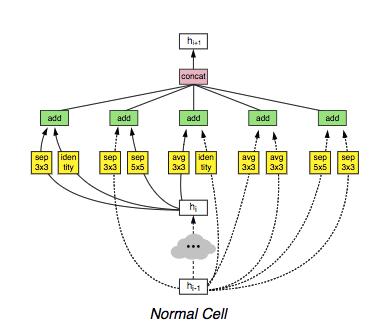
\includegraphics[width=0.5\textwidth]{NasNet.png}\hfill
  \caption{One of the basic cells of the NASNet, named the Normal Cell}
\end{figure}

First, the head layers are analyzed. It consists of a Global Average Pooling layer and a Dense layer. The Global Average Pooling layer is kept and the Dense layer is changed by a layer adapted to the new classification problem.

\begin{figure}[ht!]
  \centering
  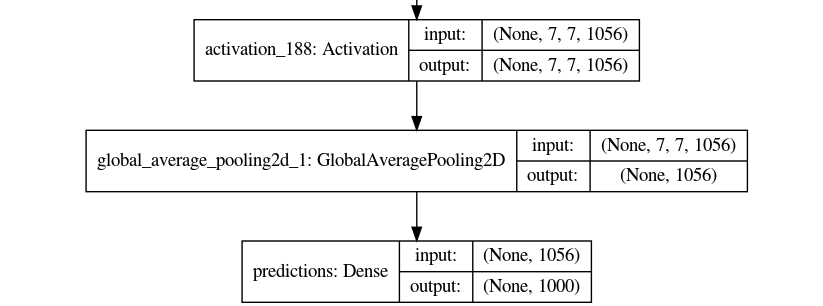
\includegraphics[width=0.5\textwidth]{last-layers.png}\hfill
  \caption{The last layers have been changed}
\end{figure}

For this task, a limitation to use only 400 images of the training set is added. The best way to overcome this limitation is the use of Data Augmentation techniques \todo{28. Cite something about Data Augmentation}.

Data Augmentation is a technique that is used to create synthetic images based on the real images that it gets in input. It is defined by a set of transformations to be applied to the training images, such as horizontal or vertical flips, shifting, rotation or zooming.

In this project, Data Augmentation is applied by using a range of 5 degrees of rotation, a horizontal and vertical shift of 0.5 and a zoom of 0.2.

The main challenge in the training or adaptation of these deep learning is to tune a set of hyper-parameter related to the training evolution (such as learning rate or momentum), regularization parameters (such as drop-out or weight decay) and choosing the right optimizer to use (RMSProp, SGD or Adam are considered). Once the new layers have been trained to adapt for the new task it may improve the performance to retrain the complete new NasNet for some epochs with a small learning rate to increase the capacity of the system.

The results obtained applying transfer learning from a NasNetMob network are \ref{TransferResults}

\todo{29. Put real results here}
\begin{table}[ht!] \label{TransferResults}
\caption{Results of Transfer Learning results.}
\begin{center}
\begin{tabular}{ | c | c | c | c | }
\hline
 & \textbf{Map at 1} & \textbf{Map a 3} & \textbf{F} \\ 
 \hline
 \textbf{Color descriptor} & 0.6 & 0.7 & 0.4 \\  
 \hline
 \textbf{LBP descriptor} & 0.7 & 0.75 & 0.5 \\ 
 \hline
 \textbf{HOG descriptor} & 0.8 & 0.85 & 0.6 \\  
 \hline
 \textbf{Combined descriptors} & 0.95 & 0.98 & 0.8 \\  
 \hline
\end{tabular}
\label{sample table}
\end{center}
\end{table}

\subsection{Design a full Convolutional Neural Network Architecture}

In this section, a procedure to design a complete neural network architecture that solves the problem in \ref{problem} is provided.

Even though the objective is to find the highest performing architecture, there is a constrain in the number of parameters of the model. 
The goal must be to keep this number as low as possible, while keeping a good enough overall system performance. Therefore, a new metric is introduced to keep track of this goal. This metric is the ratio:
%accuracy / (# parameters / 105).
\todo{30. Put this equation in an equation form}

In this procedure the same Data Augmentation logic as in \ref{transfer}.

\todo{31. POSAR TOTA LA XIXA WEEK5}

\section{Conclusions}

This document has shown the strengths and weaknesses of different machine learning models.
Classic machine learning models have been easy and quick to implement and train, but at the same time had limited capacity.
Deep learning models have been harder to tweak and were slow to train, but proved to be exceptionally good at performing the task.
It has been shown that it is possible to successfully transfer learnt features from a given task into our new task, taking advantage of work that might have been done using resources beyond the capabilities of most companies or institutions.

\todo{32. think about some other conclusions}

\bibliographystyle{splncs04}
\bibliography{bibliography.bib}
\end{document}
